% !TEX root = task-3-19-3.tex
% Editable task bank. Append new BankTask blocks at the end of the document.
\documentclass[12pt,a4paper]{article}
\usepackage{physics-textbook}
\usepackage{graphicx,needspace}
\usetikzlibrary{decorations.pathmorphing}
\newif\ifShowSolutions
\ifdefined\TutorEdition
  \ShowSolutionstrue
\else
  \ShowSolutionsfalse % Change to \ShowSolutionstrue to display solutions.
\fi
\newcounter{banktask}
\newsavebox{\BankTaskBox}
\newcommand{\BankTaskContent}[3]{%
  \noindent\textbf{\thebanktask.}\quad #2\par
  \ifShowSolutions
    \Needspace{50mm}% Keep the solution heading with its opening text or diagram.
    #3\par
    \ifdefined\TutorEdition
      \ifcsname TutorSource#1\endcsname
        \nopagebreak\smallskip{\small\csname TutorSource#1\endcsname\par}%
      \fi
    \fi
  \fi
}
\newcommand{\BankTask}[3]{%
  \refstepcounter{banktask}\par\medskip
  \sbox{\BankTaskBox}{\begin{minipage}{\linewidth}%
    \BankTaskContent{#1}{#2}{#3}\end{minipage}}%
  \ifdim\dimexpr\ht\BankTaskBox+\dp\BankTaskBox\relax>\dimexpr\textheight-20mm\relax
    \Needspace{35mm}\BankTaskContent{#1}{#2}{#3}%
  \else
    \Needspace{\dimexpr\ht\BankTaskBox+\dp\BankTaskBox\relax}%
    \noindent\usebox{\BankTaskBox}\par
  \fi
  \medskip
}
\begin{document}
\BookSubsection{3.19.3}{Закон электромагнитной индукции Фарадея}


% Source sdamgia-10473: https://phys-ege.sdamgia.ru/problem?id=10473
\BankTask{sdamgia-10473}{
За время $\Delta t$  =  $4\,\text{с}$ магнитный поток через площадку, ограниченную проволочной рамкой, равномерно уменьшается от некоторого значения \ensuremath{\Phi} до нуля. При этом в рамке генерируется ЭДС, равная $6\,\text{мВ}$. Определите начальный магнитный поток \ensuremath{\Phi} через рамку. Выразите поток в милливеберах.
}{
\smallskip\noindent\textbf{Решение}\par
ЭДС по модулю равна скорости изменения магнитного потока. Значит, изменение магнитного потока равно $6\,\text{мВ}$ · $4\,\text{с}$  =  $24\,\text{мВб}$. Поскольку конечное значение магнитного потока равно нулю, начальный магнитный поток равен $24\,\text{мВб}$.

Ответ: $24$.
}

% Source sdamgia-39925: https://phys-ege.sdamgia.ru/problem?id=39925
\BankTask{sdamgia-39925}{
Контур площадью $50\,\text{см}^{2}$ находится в однородном магнитном поле, линии индукции которого перпендикулярны плоскости контура. Чему равен модуль ЭДС индукции, возникающей в этом контуре при равномерном уменьшении модуля индукции магнитного поля от $1{,}2\,\text{Тл}$ до $0\,\text{Тл}$ за $2\,\text{с}$? Выразите ЭДС в милливольтах.
}{
\smallskip\noindent\textbf{Решение}\par
По закону электромагнитной индукции модуль ЭДС индукции равен

\[| \mathcal E _i|= \frac{|\Delta \Phi|}{\Delta t} = \frac{|\Delta B|S \cos \alpha}{\Delta t} = \frac{1{,}2 \cdot 50 \cdot 10 ^{ - 4 } \cdot \cos 0 ^\circ}{2} =3\,\text{мВ}.\]

Ответ: $3$.
}

% Source sdamgia-9507: https://phys-ege.sdamgia.ru/problem?id=9507
\BankTask{sdamgia-9507}{
В однородном магнитном поле с индукцией $40\,\text{мТл}$ находится плоский контур в виде кольца радиусом $5\,\text{см}$, изготовленный из тонкой проволоки. Сначала контур располагается так, что линии индукции магнитного поля перпендикулярны плоскости кольца. Затем кольцо поворачивают вокруг его диаметра на угол $120^\circ$. Найдите модуль изменения потока вектора магнитной индукции через кольцо при таком повороте. Выразите изменение потока в микровеберах и округлите до целого числа.
}{
\smallskip\noindent\textbf{Решение}\par
Магнитный поток через рамку равен произведению площади рамки на величину вектора магнитной индукции и на косинус угла между перпендикуляром к рамке и направлением поля:

\[\Phi =BS \cos \alpha .\]

Найдем модуль изменения потока вектора магнитной индукции:

$|\Delta \Phi| = |BS \cos \alpha _{\,\text{кон}} - BS \cos \alpha _{\,\text{нач}}|=BS | \cos 120 ^\circ - \cos 0 ^\circ |= B \pi R ^2 | \cos 120 ^\circ - \cos 0 ^\circ |=$
$=40 \cdot 10 ^{ - 3 } \cdot 3{,}14 \cdot ( 5 \cdot 10 ^{ - 2 } ) ^2 \cdot | - \frac{1}{2} - 1 | =471\,\text{мкВб}.$

Ответ: $471$.
}

% Source sdamgia-11938: https://phys-ege.sdamgia.ru/problem?id=11938
\BankTask{sdamgia-11938}{
\begin{center}\begin{tikzpicture}[x=.78cm,y=.17cm,>=stealth]
\draw[task axis] (-.68,0)--(6.08,0) node[below left] {$t,\,\text{с}$};
\draw[task axis] (0,-6.3)--(0,11.35) node[below left] {$\Phi,\,\text{Вб}$};
\draw (0,8)--(1,8)--(1,0) (0,-4)--(2,-4) (2,0)--(2,-4) (3,0)--(3,-4);
\draw[task curve,orange!85!black] (0,0)--(1,8)--(2,-4)--(3,-4)--(5,0);
\foreach \x in {1,2,3,4,5}{\node[circle,fill,inner sep=1.3pt]at(\x,0){};}
\foreach \y in {-4,4,8}{\node[circle,fill,inner sep=1.3pt]at(0,\y){};\node[left]at(0,\y){$\y$};}
\node[below left]at(0,0){$0$};
\node at(.26,5.65){$1$};\node at(1.6,5.65){$2$};
\node at(2.5,-5.55){$3$};\node at(4.17,-3.5){$4$};
\end{tikzpicture}\end{center}
На рисунке показан график зависимости магнитного потока, пронизывающего контур, от времени. На каком из участков графика ($1$, $2$, $3$ или $4$) в контуре возникает максимальная по модулю ЭДС индукции?
}{
\smallskip\noindent\textbf{Решение}\par
ЭДС по модулю равна скорости изменения магнитного потока. Чем больше скорость изменения магнитного потока, тем больше ЭДС индукции. Модуль скорости изменения магнитного потока максимален на участке $2$.

Ответ: $2$.
}

% Source sdamgia-9028: https://phys-ege.sdamgia.ru/problem?id=9028
\BankTask{sdamgia-9028}{
В опыте по наблюдению электромагнитной индукции квадратная рамка из одного витка тонкого провода находится в однородном магнитном поле, перпендикулярном плоскости рамки. Индукция магнитного поля равномерно возрастает от $0$ до максимального значения В$_{\,\text{макс}}$ за время Т. При этом в рамке возбуждается ЭДС индукции, равная $6\,\text{мВ}$. Какая ЭДС индукции возникнет в рамке, если Т уменьшить в $3$ раза, а В$_{\,\text{макс}}$ уменьшить в $2$ раза? Выразите ЭДС в милливольтах.
}{
\smallskip\noindent\textbf{Решение}\par
Величина ЭДС индукции в рамке определяется выражением:

\[\mathcal E=| \frac{\Delta \Phi}{\Delta t} |=| \frac{S\Delta B}{\Delta t} |= \frac{SB_{\,\text{макс}}}{T} .\]

Следовательно при новых параметрах будет возникать ЭДС:

\[\mathcal E_2= \frac{3}{2} \mathcal E_1=9\,\text{мВ}.\]

Ответ: $9$.
}

% Source sdamgia-46772: https://phys-ege.sdamgia.ru/problem?id=46772
\BankTask{sdamgia-46772}{
При равномерном вращении в однородном постоянном магнитном поле квадратной рамки в ней возникает ЭДС индукции, максимальная величина которой равна $2\,\text{мВ}$. Какой будет максимальная ЭДС индукции, если, не изменяя магнитное поле, каждую сторону рамки увеличить в $2$ раза, а угловую скорость вращения в $2$ раза уменьшить? Ориентация оси рамки относительно линий индукции магнитного поля не изменилась. Выразите ЭДС в милливольтах.
}{
\smallskip\noindent\textbf{Решение}\par
Максимальное значение ЭДС при вращении рамки в магнитном поле равно $\mathcal E _{\max} = BS\omega,$ где площадь рамки равна $S = a ^2 ,$ откуда $\mathcal E _{\max} = Ba ^2 \omega.$ Из анализа формулы получаем, что при увеличении стороны рамки в $2$ раза и уменьшении угловой скорости вращения в $2$ раза максимальное значение ЭДС увеличится в $2$ раза и станет равным $4\,\text{мВ}$.

Ответ: $4$.
}

% Source sdamgia-3880: https://phys-ege.sdamgia.ru/problem?id=3880
\BankTask{sdamgia-3880}{
При проведении опытов по изучению электромагнитной индукции измеряют изменение магнитного потока $\Delta \Phi,$ пронизывающего замкнутый проволочный контур, и заряд $\Delta q,$ протекший в результате этого по контуру. Ниже приведена таблица, полученная в результате этих опытов. Чему равно сопротивление контура? 

\begin{center}\begin{tabular}{|c|c|c|c|c|}\hline
$\Delta \Phi,$ Вб&$0{,}01$&$0{,}02$&$0{,}03$&$0{,}04$\\\hline
$\Delta q,$ мКл&$5$&$10$&$15$&$20$\\\hline
\end{tabular}\end{center}
}{
\smallskip\noindent\textbf{Решение}\par
Согласно закону электромагнитной индукции, величина ЭДС индукции пропорциональна скорости изменения магнитного потока через контур: 

\[\mathcal E=| \frac{\Delta \Phi}{\Delta t} |.\]

C другой стороны, по закону Ома ЭДС индукции приводит к появлению в контуре тока: $\mathcal E=IR= \frac{\Delta q}{\Delta t} R.$
Таким образом, сопротивление контура можно найти следующим образом:

\[R= \frac{\Delta \Phi}{\Delta q} = \frac{0{,}03\,\text{Вб}}{0{,}015\,\text{Кл}} =2\,\text{Ом}.\]

Ответ: $2$.
}

% Source sdamgia-7130: https://phys-ege.sdamgia.ru/problem?id=7130
\BankTask{sdamgia-7130}{
Плоская горизонтальная фигура площадью $0{,}1\,\text{м}^{2}$, ограниченная проводящим контуром, имеющим сопротивление $5\,\text{Ом}$, находится в однородном магнитном поле. Проекция вектора магнитной индукции на вертикальную ось О$_{z}$ медленно и равномерно возрастает от некоторого начального значения B$_{1z}$ до конечного значения B$_{2z}$  =  $4{,}7\,\text{Тл}$. За это время по контуру протекает заряд $\Delta q$  =  $0{,}08\,\text{Кл}$. Найдите B$_{1z}$.
}{
\smallskip\noindent\textbf{Решение}\par
По закону электромагнитной индукции модуль ЭДС индукции в случае однородного поля: $\mathcal E =| \frac{\Delta \Phi}{\Delta t} |,$ где  $\Delta \Phi=\Delta B_zS,$ а S  – площадь фигуры; $\Delta B_z=B_{2z} - B_{1z}.$
Закон Ома:  $\mathcal E = IR,$ где R  — сопротивление контура; $I= \frac{\Delta q}{\Delta t}$  — ток в контуре за время $\Delta t$ изменения магнитного поля.
Выражение для заряда, протекающего по цепи: $\Delta q = I\Delta t= \frac{S}{R} ( B_{2z} - B_{1z} ) .$

\[B_{1z}=B_{2z} - \frac{R\Delta q}{S} = 4{,}7 - \frac{5 \cdot 0{,}08}{0{,}1} =0{,}7\,\text{Тл}.\]

Ответ: B$_{1z}$ = $0{,}7\,\text{Тл}$.
}

% Source sdamgia-5737: https://phys-ege.sdamgia.ru/problem?id=5737
\BankTask{sdamgia-5737}{
Проволочная катушка сопротивлением $10\,\text{Ом}$ расположена в постоянном однородном магнитном поле так, что линии его индукции направлены вдоль оси катушки. Если соединить концы проволоки друг с другом и выключить магнитное поле, то через катушку протечет заряд $0{,}2\,\text{Кл}$. Найдите амплитуду ЭДС индукции, которая возникнет в катушке, если вновь включить прежнее магнитное поле и начать вращать в нем катушку с угловой скоростью $3\,\text{рад/с}$. Ось вращения перпендикулярна оси катушки. Ответ приведите в вольтах.
}{
\smallskip\noindent\textbf{Решение}\par
По закону Фарадея изменение магнитного потока, пронизывающего замкнутый проводящий контур, во времени, приводит к возникновению ЭДС индукции $\mathcal E_i = - \frac{\Delta \Phi}{\Delta t} .$
C другой стороны, по закону Ома ЭДС индукции выражается через силу тока в контуре и сопротивление контура
$I= \frac{\mathcal E _i}{R} .$ По определению силы тока $I= \frac{\Delta q}{\Delta t} .$
Поэтому $- \Delta \Phi = \Phi - 0 = \Delta qR.$ Здесь $\Phi$  — магнитный поток, пронизывавший катушку до выключения поля. 
При вращении катушки поток будет изменяться по закону $\Phi_1=\Phi \cos \omega t,$ следовательно: 

\[\mathcal E_i = - \Phi'_t = \Phi \omega \sin \omega t=\Delta qR\omega \sin \omega t.\]

Следоватеьно, амплитуда ЭДС индукции равна $\mathcal E_{\max}=\Delta qR\omega =0{,}2\,\text{Кл} \cdot 10\,\text{Ом} \cdot 3\,\text{рад/с}=6\,\text{В}.$

Ответ: $6\,\text{В}$.
}

% Source sdamgia-11955: https://phys-ege.sdamgia.ru/problem?id=11955
\BankTask{sdamgia-11955}{
\begin{center}\begin{tikzpicture}[>=stealth]

\draw[step=.5,gray!55] (0,-1.5)grid(3,2.5);
\draw[->] (0,-1.5)--(0,2.58) node[above left]{$B_{\text{п}},\,\text{Тл}$};\draw[->] (0,0)--(3.08,0) node[right]{$t,\,\text{с}$};
\draw[thick](0,1.5)--(1,-1)--(2.5,.5);\node[below left] at(0,0){$0$};
\foreach \y/\t in {-.5/{-0{,}2},-1/{-0{,}4},.5/{0{,}2},1/{0{,}4},1.5/{0{,}6}}{\node[left]at(0,\y){$\t$};}
\node[below]at(1,0){$4$};\node[below]at(2,0){$8$};
\end{tikzpicture}\end{center}
Квадратная проволочная рамка со стороной l  =  $10\,\text{см}$ находится в однородном магнитном поле с индукцией $\vec{B}.$ На рисунке изображена зависимость проекции вектора $\vec{B}$ на перпендикуляр к плоскости рамки от времени. Какое количество теплоты выделится в рамке за время t  =  $10\,\text{с}$, если сопротивление рамки R  =  $0{,}2\,\text{Ом}$?
}{
\smallskip\noindent\textbf{Решение}\par
При изменении магнитного поля изменяется поток вектора магнитной индукции $\,\text{Ф} ( t ) = B ( t ) S$ через рамку площадью $S = l ^2 ,$ что создает в ней ЭДС индукции $\mathcal E.$ В соответствии с законом индукции Фарадея:

\[\mathcal E = - \frac{\Delta \,\text{Ф}}{\Delta t} .\]

Эта ЭДС вызывает в рамке ток, сила которого определяется законом Ома для замкнутой цепи: 

\[I= \frac{\mathcal E}{R} .\]

Согласно закону Джоуля  — Ленца за время $\Delta$t в рамке выделится количество теплоты:

\[Q = I ^2 R\Delta t .\]

Таким образом, количество теплоты, выделяющееся в рамке, равно:

\[Q= \frac{l ^{4}}{R} \cdot \frac{( \Delta B_n ) ^2}{\Delta t} .\]

На первом участке графика $\Delta t = t_1 = 4\,\text{с}$ и $\Delta B = B_1 - B_0 = - 1\,\text{Тл},$ на втором участке $\Delta t_2 = t_2 - t_1 = 6\,\text{с}$ и $\Delta B = B_2 - B_1 = 0{,}6\,\text{Тл},$ поэтому суммарное количество выделившейся теплоты:

\[Q = Q_1 + Q_2 = \frac{l ^{4}}{R} \left[ \frac{( \Delta B_1 ) ^2}{\Delta t_1} + \frac{( \Delta B_2 ) ^2}{\Delta t_2} \right] .\]

Подставляя сюда значения физических величин, получим:

\[Q = \frac{( 0{,}1\,\text{м} ) ^{4}}{0{,}2\,\text{Ом}} \cdot \left[ \frac{1\,\text{Тл} ^2}{4\,\text{с}} + \frac{0{,}36\,\text{Тл} ^2}{6\,\text{с}} \right] = 0{,}155 \cdot 10 ^{ - 3 } \,\text{Дж}.\]

Ответ: $0{,}155\,\text{мДж}$.
}


% Source e4eF4A: https://ege.fipi.ru/bank/questions.php?search=1&proj=BA1F39653304A5B041B656915DC36B38&qid=e4eF4A
\BankTask{e4eF4A}{
За \(\Delta t=2\ \text{мс}\) магнитный поток, пронизывающий площадку, которая ограничена проводящим витком, равномерно возрастает от \(2\) до \(8\ \text{мВб}\). Чему равен модуль ЭДС индукции в витке (в $\text{В}$)?
}{
\smallskip\noindent\textbf{Решение от GPT}\par
По закону Фарадея при равномерном изменении потока
\[
|\mathcal{E}|=\frac{|\Delta\Phi|}{\Delta t}=\frac{(8-2)\cdot10^{-3}}{2\cdot10^{-3}}=3\ \text{В}.
\]
Ответ: \(3\ \text{В}\).
}

% Source F1e9FF: https://ege.fipi.ru/bank/questions.php?search=1&proj=BA1F39653304A5B041B656915DC36B38&qid=F1e9FF
\BankTask{F1e9FF}{
За промежуток времени $\Delta t$ магнитный поток, пронизывающий проволочную рамку, равномерно уменьшается от $28\,\text{мВб}$ до нуля. При этом в рамке генерируется ЭДС, равная $7\,\text{мВ}$. Определите промежуток времени $\Delta t$ (в $\text{с}$).
}{
\smallskip\noindent\textbf{Решение от GPT}\par
По закону Фарадея $|\mathcal{E}|=\dfrac{|\Delta\Phi|}{\Delta t}$. Тогда
\[
\Delta t=\frac{28\cdot10^{-3}}{7\cdot10^{-3}}=4\,\text{с}.
\]
Ответ: $4\,\text{с}$.
}

% Source 9C35AF: https://ege.fipi.ru/bank/questions.php?search=1&proj=BA1F39653304A5B041B656915DC36B38&qid=9C35AF
\BankTask{9C35AF}{
В опыте по наблюдению электромагнитной индукции квадратная рамка из одного витка тонкого провода находится в однородном магнитном поле, перпендикулярном плоскости рамки. Индукция магнитного поля равномерно возрастает от $0$ до максимального значения $B_{\text{макс}}$ за время $T$. При этом в рамке возбуждается ЭДС индукции, равная $6\,\text{мВ}$. Какая ЭДС индукции (в $\text{мВ}$) возникнет в рамке, если $T$ уменьшить в $3$ раза, а $B_{\text{макс}}$ уменьшить в $2$ раза?
}{
\smallskip\noindent\textbf{Решение от GPT}\par
Модуль ЭДС равен $|\mathcal{E}|=S B_{\text{макс}}/T$. Поэтому
\[
|\mathcal{E}'|=\frac{S(B_{\text{макс}}/2)}{T/3}=\frac32|\mathcal{E}|=9\,\text{мВ}.
\]
Ответ: $9\,\text{мВ}$.
}

% Source 9FB8B0: https://ege.fipi.ru/bank/questions.php?search=1&proj=BA1F39653304A5B041B656915DC36B38&qid=9FB8B0
\BankTask{9FB8B0}{
На рисунке показан график зависимости магнитного потока $\Phi$, пронизывающего контур, от времени $t$. Найдите модуль ЭДС индукции (в $\text{В}$) в контуре в промежутке времени от $2$ до $4\,\text{с}$.
\begin{center}
\begin{tikzpicture}[x=0.55cm,y=0.275cm,>=stealth]
\draw[->] (0,-9.2)--(0,11.8);
\draw[->] (0,0)--(11.8,0);
\node[above left] at (0,10.5) {$\Phi,\,\text{Вб}$};
\node[below] at (11.5,-0.5) {$t,\,\text{с}$};
\foreach \x in {2,4,6,8,10}{\draw (\x,-0.55)--(\x,0.55);\node[below] at (\x,-0.55) {$\x$};}
\foreach \y in {-8,-4,4,8}{\draw (-0.22,\y)--(0.22,\y);\node[left] at (-0.3,\y) {$\y$};}




\draw (3.25,4)--(4.85,4);
\draw (6.45,4)--(8.1,4);
\draw (9.75,4)--(10,4);
\draw (0,-8)--(.8,-8);
\draw (2.45,-8)--(4,-8);
\draw (2,-.8)--(2,4);
\draw (4,-8)--(4,-4.9);
\draw (10,.25)--(10,3.3);
\draw[thick] (0,4)--(2,4)--(4,-8)--(6,0)--(10,4);
\end{tikzpicture}
\end{center}
}{
\smallskip\noindent\textbf{Решение от GPT}\par
На участке от $2$ до $4\,\text{с}$ поток равномерно изменяется от $4$ до $-8\,\text{Вб}$. По закону Фарадея
\[
|\mathcal{E}|=\frac{|\Delta\Phi|}{\Delta t}=\frac{|-8-4|}{4-2}=6\,\text{В}.
\]
Ответ: $6\,\text{В}$.
}

% Source 7FABFc: https://ege.fipi.ru/bank/questions.php?search=1&proj=BA1F39653304A5B041B656915DC36B38&qid=7FABFc
\BankTask{7FABFc}{
За время $\Delta t=2\,\text{с}$ магнитный поток через площадку, ограниченную проволочной рамкой, равномерно уменьшается от некоторого значения $\Phi$ до нуля. При этом в рамке генерируется ЭДС индукции, равная $10\,\text{мВ}$. Определите начальный магнитный поток $\Phi$ через рамку. (в $\text{мВб}$).
}{
\smallskip\noindent\textbf{Решение от GPT}\par
По закону Фарадея $|\mathcal E|=|\Delta\Phi|/\Delta t=\Phi/\Delta t$. Поэтому $\Phi=|\mathcal E|\Delta t=10\cdot10^{-3}\cdot2=0{,}020\,\text{Вб}=20\,\text{мВб}$. Ответ: $20\,\text{мВб}$.
}

% Source F4BE25: https://ege.fipi.ru/bank/questions.php?search=1&proj=BA1F39653304A5B041B656915DC36B38&qid=F4BE25
\BankTask{F4BE25}{
На железный сердечник надеты две катушки, как показано на рисунке. По правой катушке пропускают ток, который меняется согласно приведённому графику.
\begin{enumerate}
\item В промежутках времени $0\text{–}1\,\text{с}$ и $3\text{–}5\,\text{с}$ направления тока в левой катушке одинаковы.
\item В промежутке времени $2\text{–}3\,\text{с}$ сила тока в левой катушке равна $0$.
\item Модули силы тока в левой катушке в промежутках времени $1\text{–}2\,\text{с}$ и $3\text{–}5\,\text{с}$ одинаковы.
\item В промежутке $0\text{–}2\,\text{с}$ модуль индукции магнитного поля в сердечнике равен $0$.
\item В левой катушке сила тока в промежутке времени $0\text{–}1\,\text{с}$ по модулю больше, чем в промежутке времени $3\text{–}5\,\text{с}$.
\end{enumerate}
\begin{center}
\begin{tikzpicture}[book diagram,x=1cm,y=1cm]
\draw (0,0.8) rectangle (4.4,2.25);
\foreach \x in {0.25,0.35,...,1.75}{
\draw[line width=0.3pt] (\x,0.8) .. controls (\x-0.15,1.15) and (\x-0.10,1.90) .. (\x+0.10,2.25);
\draw[line width=0.3pt] (\x+0.10,2.25) .. controls (\x+0.24,2.55) and (\x+0.25,2.33) .. (\x+0.18,2.15);
\draw[line width=0.3pt] (\x+0.18,2.15) .. controls (\x+0.01,1.55) and (\x+0.01,1.00) .. (\x+0.10,0.8);
}
\foreach \x in {2.5,2.6,...,4.0}{
\draw[line width=0.3pt] (\x,0.8) .. controls (\x-0.15,1.15) and (\x-0.10,1.90) .. (\x+0.10,2.25);
\draw[line width=0.3pt] (\x+0.10,2.25) .. controls (\x+0.24,2.55) and (\x+0.25,2.33) .. (\x+0.18,2.15);
\draw[line width=0.3pt] (\x+0.18,2.15) .. controls (\x+0.01,1.55) and (\x+0.01,1.00) .. (\x+0.10,0.8);
}
\draw (0.25,0.8)--(0.25,0.05);
\draw (0.25,-0.12) rectangle (0.98,0.22);
\draw (0.98,0.05)--(1.16,0.05);
\draw (1.49,0.05) circle[radius=0.33];
\node at (1.49,0.05) {$\mathrm{A}$};
\draw (1.82,0.05)--(1.90,0.05)--(1.90,0.8);
\draw (2.5,0.8)--(2.5,0.05)--(3.04,0.05);
\draw (3.12,0.05) circle[radius=0.065];
\draw (3.62,0.05) circle[radius=0.065];
\draw (3.69,0.05)--(4.16,0.05)--(4.16,0.8);
\draw (3.02,-0.07)--(3.22,0.17);
\draw (3.52,-0.07)--(3.72,0.17);
\end{tikzpicture}

\begin{tikzpicture}[book diagram,x=0.65cm,y=0.325cm]
\draw[xstep=0.5,ystep=1,gray,very thin] (0,-4) grid (5,4);
\draw[-{book tip}] (0,-5.2)--(0,5.9);
\draw[-{book tip}] (0,0)--(6,0);
\node[above left] at (0,5.1) {$i,\,\text{А}$};
\node[below right] at (5.7,-0.05) {$t,\,\text{с}$};
\foreach \x in {1,2,3,4,5}{\node[below,fill=white,inner sep=1pt] at (\x,0) {$\x$};}
\foreach \y in {-4,-2,0,2,4}{\node[left] at (0,\y) {$\y$};}
\draw[thick] (0,-4)--(2,4)--(3,4)--(5,0);
\end{tikzpicture}
\end{center}
}{
\smallskip\noindent\textbf{Решение от GPT}\par
Индукционный ток в левой катушке определяется изменением потока: $\mathcal E=-M\,\Delta i/\Delta t$, поэтому его модуль пропорционален модулю наклона графика. На участках $0$–$2\,\text{с}$ и $3$–$5\,\text{с}$ наклоны равны соответственно $4\,\text{А/с}$ и $-2\,\text{А/с}$: направления индукционного тока противоположны, а модули отличаются вдвое, поэтому утверждения 1 и 3 неверны, 5 верно. На участке $2$–$3\,\text{с}$ ток правой катушки постоянен, индукционный ток отсутствует: утверждение 2 верно. На участке $0$–$2\,\text{с}$ магнитная индукция не равна нулю на всём промежутке, поскольку ток обращается в нуль только при $t=1\,\text{с}$: утверждение 4 неверно. Ответ: 2, 5.
}

% Source 2928: https://phys-ege.sdamgia.ru/problem?id=2928
\BankTask{2928}{
На рисунке приведена электрическая цепь, состоящая из гальванического элемента, реостата, трансформатора, амперметра и вольтметра.
\begin{center}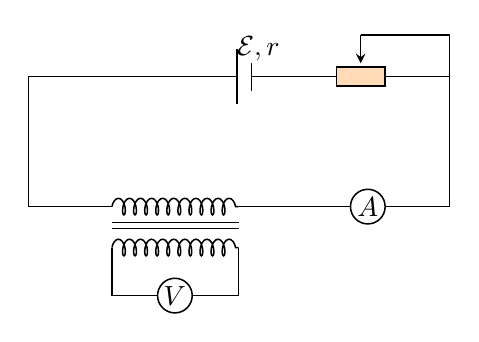
\begin{tikzpicture}[>=stealth,line width=.55pt]\draw(0,0)--(0,1.65)--(2.65,1.65) (2.83,1.65)--(5.35,1.65)--(5.35,0)--(2.67,0) (1.06,0)--(0,0);\draw(2.65,1.3)--(2.65,2) (2.83,1.47)--(2.83,1.83);\node[above]at(2.92,1.72){$\mathcal E,r$};\draw[->](4.22,2.18)--(4.22,1.82);\draw(4.22,2.18)--(5.35,2.18)--(5.35,1.65);\draw[decorate,decoration={coil,aspect=.45,amplitude=3pt,segment length=4pt}](1.06,0)--(2.67,0);\draw(1.06,-.2)--(2.67,-.2) (1.06,-.28)--(2.67,-.28);\draw[decorate,decoration={coil,aspect=.45,amplitude=3pt,segment length=4pt}](1.06,-.52)--(2.67,-.52);\draw(1.06,-.52)--(1.06,-1.13)--(2.67,-1.13)--(2.67,-.52);\draw[fill=orange!28](3.9099999999999997,1.5299999999999998)rectangle(4.529999999999999,1.77);\node[above]at(4.22,1.77){$$};\draw[fill=white](4.31,0)circle(.22)node{$A$};\draw[fill=white](1.86,-1.13)circle(.22)node{$V$};\end{tikzpicture}\end{center}
В начальный момент времени ползунок реостата установлен посередине и неподвижен. Опираясь на законы электродинамики, объясните, как будут изменяться показания приборов в процессе перемещения ползунка реостата вправо. ЭДС самоиндукции пренебречь по сравнению с $\mathcal E.$
}{
\smallskip\noindent\textbf{Решение}\par
$1$.  Во время перемещения движка реостата показания амперметра будут плавно уменьшаться, а вольтметр будет регистрировать напряжение на концах вторичной обмотки. Примечание: для полного ответа не требуется объяснения показаний приборов в крайнем правом положении. (Когда движок придет в крайнее правое положение и движение его прекратится, амперметр будет показывать постоянную силу тока в цепи, а напряжение, измеряемое вольтметром, окажется равным нулю.)
$2$.  При перемещении ползунка вправо сопротивление цепи увеличивается, а сила тока уменьшается в соответствии с законом Ома для полной цепи: $I= \frac{\mathcal E}{R + r} ,$ где R  — сопротивление внешней цепи.
Изменение тока, текущего по первичной обмотке трансформатора, вызывает изменение индукции магнитного поля, создаваемого этой обмоткой. Это приводит к изменению магнитного потока через вторичную обмотку трансформатора. В соответствии с законом индукции Фарадея возникает ЭДС индукции $\mathcal E = - \frac{\Delta \Phi}{\Delta t}$ во вторичной обмотке, а следовательно, напряжение U  на ее концах, регистрируемое вольтметром.
}

\end{document}
